\boldchapter{Transcription Termination} \label{termination}
%do writing new stuff in the morning, fixing in the afternoon.
%reset in case acronyms are cited previously, this is their main paragraph and the acronym needs to be in long form.
\glsreset{cpf}
\glsreset{nns}
After its synthesis and maturation are complete, the nascent RNA molecule must be released from the DNA template, and the elongation complex must be disassembled and its components recycled.
In \cer{}, transcription termination is enacted by several widely different mechanisms.
Two predominating pathways terminate the vast majority of transcripts generated by \acrlong{pol2}: the \gls{cpf} pathway and the \gls{nns}  pathway. 
Both these mechanisms rely on short sequences on the nascent RNA---coupled with specific modifications on the \gls{ctd} of \gls{pol2}---to recruit specific factors and enact the disassembly of the elongation complex and the release of the transcript in the nucleus.

In addition to the two main pathways cited above, several non-canonical termination mechanism have been described.x
these mechanisms are dedicated to the termination of specific RNA species, or can act as backups when the main pathways fail.


Finally, transcription termination is strictly intertwined with some steps of 3' end processing and maturation, strongly influencing the fate of the transcript. 
%The \gls{cpf} complex couples termination with a polyadenylation step and export competence of the RNA was shown to require this termination mechanism. 
%On the other hand, \gls{nns} is known to lead to either processing (for certain species such as \gls{sns} and \gls{snos}) or complete degradation of the transcript.



\section{The CPF-CF pathway}
The \gls{cpf} pathway was the first termination mechanism described in \cer{} because of its association with the termination of protein-coding genes\footnote{Its activity can extend to certain kinds of non-coding transcripts as well (see chapter \ref{pervasiveTranscripts} for details)}. 
\gls{cpf} termination is unique as it results in cleavage of the nascent RNA before termination occurs.
The site of cleavage is specified through sequence elements present on the nascent RNA and plays an important role in kickstarting the termination reaction.

The main actor of this termination mechanism is the \gls{cpf} complex, a large assembly of modular sub-complexes that act in concert to execute all the required steps. 
This complexity makes \gls{cpf} the most reliable, efficient, and precise termination mechanism in \cer{}.

%There exist some controversy about how \gls{cpf} termination mechanistically occurs.
%The literature proposes two models that explain termination through the \gls{cpf} pathway.
%The allosteric model argues that transcription through the cleavage site leads to conformational changes in the elongation complex, leading to destabilization of the complex and eventually termination.
%On the other hand, the torpedo model posits that after cleavage, the uncapped 5' end of the polymerase-associated transcript is attacked by exonuclease Rat1, leading to the dismantling of the complex through destabilization of the ternary complex once Rat1 catches up with the polymerase.



\subsection{Recruitment and assembly}
%TODO{figure}
Recruitment and initial assembly of the \gls{cpf} complex onto the nascent RNA is promoted by two mechanisms: interaction with specific sequences elements, and interaction with the polymerase \gls{ctd}.

A key component of the \gls{cpf} complex, Pcf11, contains a peptide sequence able to recognize the \gls{ctd}. This \gls{cid} is able to specifically recognize the \sert{}-phosphorylated version of the heptapeptide.
Given the nature of this \gls{ctd} modification---which is confined to the later stages of transcription---density of the \gls{cpf} complex around the polymerase is selectively increased where the complex is more likely to be needed for termination (i.e. at the 3' end of transcription units), facilitating the eventual binding of \gls{cpf} to the sequence elements on the nascent RNA.

Unlike in human, where the cleavage site is defined by a single highly conserved hexanucleotide sequence on the nascent RNA, Yeast \gls{cpf} complex recognizes a number of degenerate short sequences.
Two sub-complexes of \gls{cpf}, \gls{cf1a} and \gls{cf1b}, are responsible for the recognition of these sequences.
In particular, Rna15 and Hrp1 (components of \gls{cf1a} and \gls{cf1b} respectively) directly bind the nascent RNA.
Associated factors Rna14 and Pcf11 contribute to the assembly of the whole complex by interacting with \gls{pol2} and forming a scaffold that serves to tether the catalytic portion of the \gls{cpf} complex to the cleavage site.

The bulk of the catalytic activity of the \gls{cpf} complex is contained in the \gls{cpfa} sub-complex.
\gls{cpfa} directly contacts the cleavage site with its Ysh1 subunit and is responsible of the cleavage of the nascent RNA, one of the events that is thought to kickstart the termination reaction.
\gls{cpfa} also coordinates the polyadenylation reaction through the subunits Yth1 and Fip1. 
These factors recruit and tether the poly(A) polymerase Pap1 to the complex, which will begin catalyzing the addition of a poly(A) tail after the transcript has been cleaved.

Despite the wealth of knowledge available on the mechanics of \gls{cpf} recruitment and assembly, some controversy still surrounds the actual termination mechanism.
Two main models describing the termination reaction exist in the literature, the allosteric model and the torpedo model.

\subsection{The allosteric model}

After cleavage and release of the nascent RNA, the elongation complex has successfully accomplished its job in the transcriptional process and is ready to be disassembled.
The allosteric model is one of the two main mechanistic models that describes the process by which the \gls{tec} is removed from the DNA template.

The allosteric model argues that cleavage is a dispensable signal, and that termination can happen independently of this step.
It posits that after transcription of the cleavage site, \gls{pol2} loses a lot of factors that qualify the elongation complex as such.
Loss of these ``anti-termination" factors---components of the elongation complex that would prevent termination from occurring---would trigger conformational changes, destabilize the polymerase, and allow components of the \gls{cpf} complex itself to elicit the disassembly of \gls{pol2} from the template.

Several studies support this model. 
\gls{pol2} was shown to lose a number of associated elongation factors after reaching the 3' end \citep{kim:2004:transitions}.
In addition, the component of the \gls{cpf} complex Pcf11 was shown to be able to terminate the polymerase \invitro{} by binding the nascent RNA and the \sert{}-phosphorylated moiety of \gls{pol2} \citep{zhang:2005:ctddependent}.
Ulterior support to this last study was provided by the same authors two years later, when they discovered that Pcf11 is able to perform the same feat in drosophila \citep{zhang:2006:pcf11}.
Finally, a very recent study published on Molecular Cell was able to reconstitute transcription termination in an \invitro{} system in the absence of cleavage \citep{zhang:2015:polya}.

\subsection{The torpedo model}



According to the torpedo model, cleavage represents the main termination signal for the \gls{cpf} complex, as it leaves an uncapped 5'-P on the transcript associated with the still transcribing elongation complex.
These unprotected 5' is the substrate of \FtoT{} exonucleases, a class of enzymes that are known to progressively degrade RNA polypeptides.
The \FtoT{} exonuclease Rat1 was discovered to be associated with the \gls{cpf} complex and is thought to attack the 5' moiety of the \gls{pol2}-associated transcript, starting a processivity race with \gls{pol2}.
Upon winning the race, Rat1 would destabilize the structure of the ternary complex within the polymerase, causing it to break apart and detach from the DNA template.

There are several lines of evidence that support this model for \gls{cpf} transcription termination.
Both Rat1 and its human homolog Xrn2 exhibit termination defects in model cases when mutated \citep{kim:2004:yeast, west:2004:human}.
Furthermore, Rat1 and its co-factor Rtt103 were found to be strongly associated with the 3' end of genes and in physical association with the \gls{cpf} complex \citep{kim:2004:yeast,luo:2006:role}, supporting the idea of a functional recruitment to zones of active transcription termination.
Homology studies found that homologs of Rtt103 in both humans and \cele{} have roles in transcription termination \citep{morales:2014:kub5hera, cui:2008:genes}.
Finally, recent mechanistic studies \invivo{} have demonstrated the kinetic competition between Rat1 and the elongation complex. By employing mutant polymerases that elongate faster or slower than the wild type version, the authors were able to show that slower polymerases result in earlier termination, consistent with the notion that Rat1 needs to physically catch up with the polymerase in order to elicit termination \citep{fong:2015:effects}.

At the same time, several reports argue against the torpedo model as sole effector of transcription termination.
\Invitro{} studies were unable to reproduce the termination effect observed \invivo{} using only Rat1  \citep{dengl:2009:torpedo}. More recent ventures re-attempted the \invitro{} approach with limited success  \citep{park:2015:unraveling}, but managed to demostrate that Rat1 is able to terminate polymerases that are destabilized by nucleotide misincorporation.
Several additional mechanistic studies showed that the exonucleolytic activity of Rat1 is unable to mediate the release of the polymerase from the template \citep{luo:2006:role, pearson:2013:dismantling}.
Moreover, termination defects caused by Rat1 mutants were not associated with stabilization of the \gls{pol2}-associated transcript, arguing against the model.
%Finally, recent genome-wide studies were unsuccessful in detecting a widespread effect of Rat1 human homolog (Xrn2) in transcription termination\citep{nojima:2015:mammalian}.


\begin{figure}[ht]

\centering
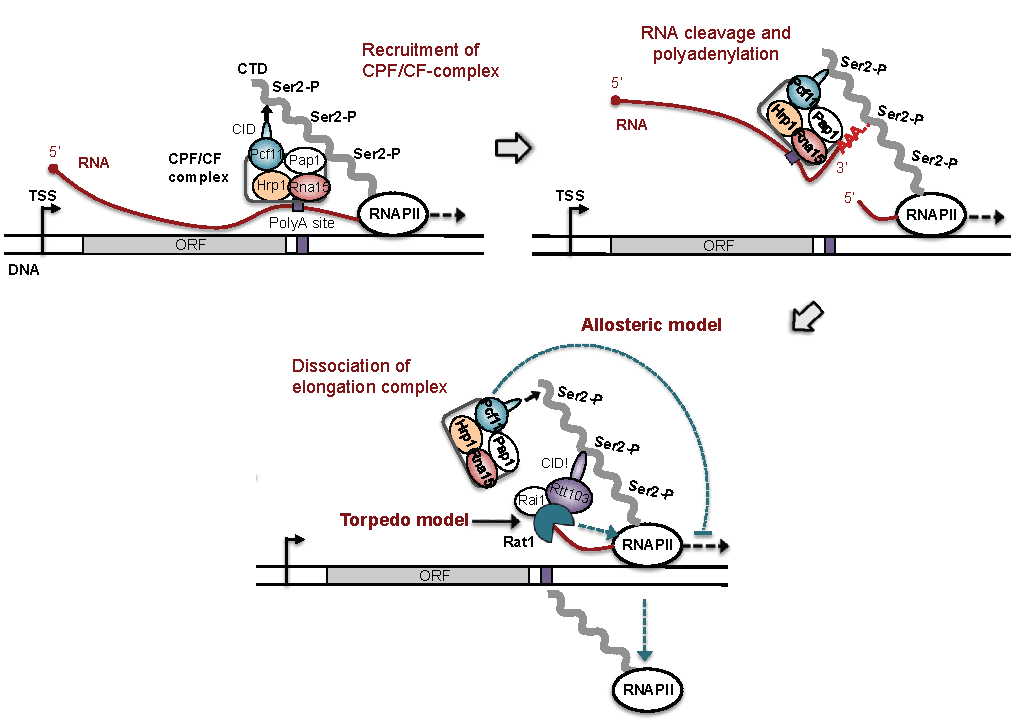
\includegraphics[width=\textwidth]{figures/introduction/cpf}
\caption[Mechanism of CPF-CF termination]{Overview of the main mechanistic step that lead to CPF-CF termination. The complex is recruited thanks to CTD phosphorylation and binding sites on the RNA. The transcript is then cleaved and the elongation complex terminated in accordance with the torpedo or allosteric model.}
\label{fig:cpfTermination}

\end{figure}

\subsection{A unified view of CPF-CF transcription termination}

As evidence for and against the two models piles up, a unified view that combines elements of both torpedo and allosteric model is taking shape.
While the effect of Rat1 on transcription termination (of at least some transcripts) is established, its role as main effector of \gls{cpf} termination has been repeatedly called into question.
Several studies have now described interdependencies between Rat1 and other subunits of the \gls{cpf} complex---notably Pcf11---and the perceived nature of Rat1 is shifting towards that of a molecular effector  that is integrated into a larger system.
The proof of principle that termination is possible without cleavage has been recently provided---albeit \invitro{} \cite{zhang:2015:polya}---and presence of Rat1 has been convincingly shown to facilitate termination \cite{fong:2015:effects}, arguing for a model that integrates these two mechanisms.

%Despite recent advances and the rise of a unified model for transcription termination, mechanistic details on the termination reaction and what prompts it are still sorely lacking.



\section{The NNS pathway}

NNS dependent transcription termination is the second of the main termination mechanisms in S.cerevisiae. 
It is essentially involved in the termination of small Nuclear RNAs (snRNAs), small Nucleolar RNAs (snoRNAs) and a number of other non-functional non-coding RNAs.
It sets itself apart from CPF-CF termination in a number of ways.
First and foremost, it relies on a completely different---and much smaller---set of proteins: the two RNA binding proteins Nrd1 and Nab3 \cite{conrad:2000:yeast}, together with the helicase Sen1. 
Because of the different molecular effectors, the termination mechanism---although still not fully elucidated---is appreciably different. 
Termination is not associated to cleavage of the nascent RNA, and release of the transcript occurs upon disassembly of the elongation complex itself \cite{steinmetz:2001:rnabinding}. 
As a consequence, the 3’ end of the terminated transcript coincides with the termination sites on DNA. 
The NNS complex also distinguishes itself because of the different fate imposed on the RNA released: instead of being exported to the cytoplasm after polyadenylation, the transcripts released are subjected to the activity of degradation enzymes (the nuclear exosome, see below) \cite{vasiljeva:2006:nrd1}. 
To this end the NNS complex recruits both the nuclear exosome and a specific set of 3' end processing factors known as TRAMP (Trf4/Air2/Mtr4p Polyadenylation), which drives polyadenylation and stimulates degradation \cite{lacava:2005:rna, vasiljeva:2006:nrd1}.

NNS termination operates mainly on non-coding RNAs and is generally restricted to the early stages of transcription elongation. 
Despite not being directly involved in the termination of protein-coding genes, it can play a role in the regulation of gene expression by acting as an attenuator \cite{arigo:2006:regulation}(i.e. terminating some transcription events, preventing them from producing functional RNAs), like in the case if IMD2 or URA2 genes \citep{jenks:2008:properties}, or otherwise terminating transcription of non-coding RNAs that might be involved in regulation \cite{thompson:2007:cytoplasmic}.



\subsection{The NNS complex}

The main molecular effectors of the NNS complex are the three protein Nab3, Nrd1, and Sen1.


\paragraph{Nab3}

This factor was originally identified as a polyadenylated RNA binding protein. 
Nab3 contains several structural domains: a conserved RNA Recognition Motif (RRM) that can contact specific sequence elements on the nascent RNA, a region necessary for the interaction with Nrd1, and an essential Glutammine/Proline region at the C-terminus.

Biochemical experiments have shown that Nab3 forms a stable heterodimer with Nrd1 and contacts the RNA as such \cite{conrad:2000:yeast}. 
In addition, the structure of the RRM has been solved, revealing the structural basis for the preference of the sequence UCUUG \cite{lunde:2011:structural}. 
Finally, its Glutammine/Proline region---despite being generally unstructured---can assemble into amyloid structures \cite{orourke:2015:amyloidlike}.


\paragraph{Nrd1}

Identified as part of the ``nuclear pre-mRNA downregulation" family of proteins, Nrd1 is the most abundant of the three members of the complex. 
Its main features consist of an RRM structure that allows it to contact the nascent RNA, a CTD interaction domain (CID) that mediates the interaction with RNAPII (see below) and a Nab3 interaction motif that allows it to form a stable heterodimer.

Nrd1's RRM was shown \invivo{} to contact the consensus sequence GTA[A/G] \cite{steinmetz:1998:control}. 
Recent \invitro{} studies, however, have shown that several other G-rich and A-rich sequences could be bound equally well \citep{bacikova:2014:structure}, although the \invivo{} relevance of these studies remains to be demonstrated. 

In addition to the RNA, Nrd1 can contact RNAPII through its CID \cite{kubicek:2012:serine,vasiljeva:2008:nrd1nab3sen1}. 
Although dispensable for cell viability, the CTD-CID interaction is required for efficient termination (see below).

Curiously, Nrd1 also contains a Glutammine/Proline region at the C-terminus, similarly to Nab3. 
Deletion of this region shows no growth or termination defects, but is synthetic lethal if combined with other aphenotypic mutations on Nab3 [our unpublished data]. 
The functional implications of these genetic interactions are still unknown.
 

\paragraph{Sen1}

This extremely large (253kDa) and very low abundance (125 molecules per cell) protein is the only member of the NNS complex to have enzymatic activity \cite{steinmetz:1996:repression}. 
Sen1 was characterized as a helicase of the SFI superfamily and is very closely related to Upf1, a member of the Non-sense Mediated mRNA Decay (NMD) pathway in the cytoplasm. 
Unlike its close relative, Sen1 possesses a nuclear localization signal and acts in the nucleus, where it can physically interact with the other members of the NNS complex Nrd1 and Nab3. 

Structurally, Sen1 contains a helicase domain able to hydrolize ATP and a large N terminal domain. 
The helicase domain was recently purified in E.coli and biochemically analyzed, revealing binding affinity for both DNA and RNA, but a slower translocation rate on RNA \cite{martintumasz:2015:saccharomyces}. 
Moreover, its ATPase activity was shown to be necessary for termination \invitro{} \cite{porrua:2013:bacteriallike}. 
The N-terminal region of Sen1 was implicated in the interaction with the RNAPII, as well as other factors such as Rnt1 and Rad2, but the implications of the latter interactions remain obscure.

\subsection{The mechanism of transcription termination}

As in the case of CPF-CF, the NNS complex is recruited to the region of termination through two distinct mechanisms that cooperate to maximize efficiency: the CTD of the polymerase \cite{vasiljeva:2008:nrd1nab3sen1} and specific sequence elements on the nascent RNA \cite{conrad:2000:yeast}. 
Within the NNS complex, Nrd1 and Nab3 are the major interactors of these elements, providing specificity and ensuring that Sen1---believed to be the molecular effector of NNS termination---is recruited only in the appropriate circumstances \cite{porrua:2013:bacteriallike}.

The CTD of RNAPII is contacted by the CID domain of Nrd1. 
This domain preferentially recognizes the Ser5-phosphorylated variant, which is the prevalent CTD phosphorylation state in the first 500-600 nucleotides of transcription. 
This preference confers to the NNS complex a high degree of specificity for terminating transcription in the early stages of elongation. 
According to the current model for NNS termination, the interaction with the CTD occurs prior to RNA binding, and facilitates recognition of sequence elements on the nascent transcript.  
Presence of Ser5-P CTD was shown to be a pre-requisite for efficient termination, as placing high efficiency NNS binding sites at the end of long transcription units---where the levels of Ser5-P would be completely supplanted by Ser2-P---does not result in termination \cite{gudipati:2008:phosphorylation}.

\begin{figure}[ht]

\centering
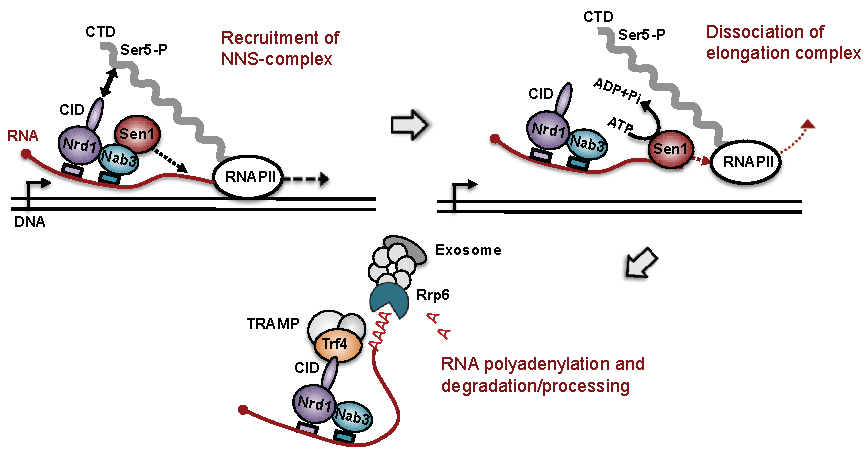
\includegraphics[width=\textwidth]{figures/introduction/nns}
\caption[Mechanism of NNS termination]{Main stages of NNS-dependent termination. the NNS complex is recruited thanks to \serf{}-phosphorylated CTD and sequence elements on the transcript. Termination is elicited by Sen1, presumably by translocating along the transcript. Finally, the exosome is recruited to the transcript and the transcript is either trimmed or completely degraded.}
\label{fig:nnsTermination}

\end{figure}

Recruitment of Nrd1 to the CTD, however necessary, is not sufficient to trigger termination. 
The Nrd1-Nab3 heterodimer must also contact the nascent RNA through the RRM domains of the two subunits.
Original studies have investigated the sequence elements that drive NNS termination, pinpointing two core consensuses: UCUU as the main binding site for Nab3, and GUA[A/G] as the main site for Nrd1 \cite{carroll:2004:identification}. 
More recent investigations redefined these consensuses and identified new sequence elements that can increase termination efficiency when in proximity of canonical binding sites. 
Use of an \invivo{} SELEX (Systematic Evolution of Ligands by Exponential enrichment) strategy allowed to extend the core consensus sequences for both Nrd1 and Nab3 with nucleotides that proved critical for binding (see fig ??) \cite{porrua:2012:in}. 
In addition, AU-rich sequences found downstream of Nrd1 sites were shown to play a role in increasing both termination efficiency and recruitment of Nrd1 \cite{porrua:2012:in}. Similar conclusions have been reached by \invivo{} crosslinking studies \cite{wlotzka:2011:nuclear}.

Despite the efforts expended in identifying sequence elements that could univocally lead to NNS termination, a lot of ambiguity remains on what constitutes an NNS terminator \invivo{}. 
While presence of Nrd1-Nab3 binding sites is required, no consistent pattern emerges in number, spacing, or quality of Nrd1/Nab3 sites at known NNS termination sites. 
Despite this, \invitro{} studies on model cases have identified some features of heterodimer binding. 
For example, mutation of Nab3 binding sites proved to be more deleterious to heterodimer recruitment than mutation of Nrd1 sites \cite{carroll:2007:interaction}. 
Moreover, multiple heterodimers were found to bind the same RNA sequence, possibly cooperatively  \cite{carroll:2007:interaction}. 
It remains impossible, however, to generalize these results beyond the few sequences tested. 
While the NNS complex could simply rely on a high number of low affinity sites to reach an occupancy threshold, it remains possible that several unseen elements play a role in qualifying NNS terminators, influencing the quantity and quality of Nrd1 and Nab3 binding sites necessary for an efficient termination.

When the Nrd1-Nab3 heterodimer is bound to the nascent RNA, the molecular effector of NNS termination, the helicase Sen1, is recruited to the complex. 
Studies have shown that Sen1 is strictly required to terminate transcription, but the mechanism through which this happens is not clear. 
Significant advances in the understanding of this phenomenon came from use of an \invitro{} transcription termination system \cite{porrua:2013:bacteriallike}. 
In this context, Sen1 alone was found to be sufficient to disassemble the elongation complex. Termination was shown to occur preferentially at sites of pausing and to require both the interaction of Sen1 with the nascent transcript and ATPase activity. 
It is unclear whether ATP-dependent translocation of Sen1 on the nascent RNA is required for termination. However, results from an \invivo{} study suggest the existence of a kinetic competition between transcription elongation and Sen1 translocation on the RNA. 
The authors investigated the effect of the speed of transcription on NNS termination, showing that faster transcription results in longer NNS-terminated transcripts, while slower transcription produces shorter transcripts and is able to suppress mutations on Sen1 \cite{hazelbaker:2013:kinetic}. 
Taken together, these results support a model where, akin to the bacterial termination factor Rho, Sen1 would contact the nascent transcript and translocate in a 5’ to 3’ direction, eliciting termination upon catching up with the polymerase.

\subsection{Processing of products of the NNS pathway}

The process of NNS termination is strictly connected with 3' end processing or degradation mediated by the nuclear exosome, a multiprotein complex endowed with exonuclease activity \cite{vasiljeva:2006:nrd1}. 
The exosome plays a major role in nuclear RNA quality control, degrading aberrant transcripts, a number of non-functional non-coding RNAs, and trimming the precursors of functional small non-coding RNAs such as sn/snoRNA \cite[for review see][]{kilchert:2016:regulation}. 
The exosome is composed of six non-catalytic subunits arranged in a ring-like structure, together with three cap subunits that can bind RNA (see figure X). 
The catalytic activity of this complex is dependent on two active 3' to 5' exonuclease, Dis3 and Rrp6. 
Dis3 associates with the ring on the opposite side of the three cap subunits, and degrades RNAs that are threaded through the cap proteins and into the ring \cite{makino:2015:rna}. 
The exosome is present throughout the nucleus and in the cytoplasm. 
However, only the nuclear version can associate with the other exonuclease, Rrp6, whose activity is known to regulate the levels of many NNS targets.

Recruitment of the exosome to NNS targets takes place via one of the exosome’s co-factors: the TRAMP complex. 
TRAMP (for Trf4/Air2/Mtr4p Polyadenylation) is a nuclear complex composed of the poly(A) polymerase Trf4, the RNA-binding protein Air2 and the helicase Mtr4. 
Trf4 is the core subunit of the complex, to which both Air2 and Mtr4 bind independently. 
It possesses poly(A) polymerase activity, but unlike Pap1---the canonical poly(A) polymerase associated with the CPF-CF complex---it can only add tails in a distributive manner. 
Trf4 is also the factor responsible for the coordination between the NNS complex and the nuclear exosome. 
A recent study showed that Trf4 contacts Nrd1 through a small motif called Nrd1 Interaction Motif (NIM) . 
The NIM on Trf4 mimicks Ser5-P CTD and can therefore compete with the CTD of RNAPII for the interaction with the CID (CTD interaction domain) on Nrd1. 
The interaction of Nrd1’s CID with the CTD and Trf4 are mutually exclusive, and Trf4 was shown to have much higher affinity for the CID. 
These findings have suggested a model whereby TRAMP is recruited to the RNA when the CID of Nrd1 is freed from the CTD of the polymerase \cite{tudek:2014:molecular}. 
This effectively allows the coordination of events going from termination to the handover of the transcript to TRAMP and the exosome.

As a co-factor of the exosome, TRAMP is able to both recruit and stimulate its activity. 
Addition of a poly(A) tail to the terminated transcript is thought to provide an unstructured platform that can be easily be threaded through the non-catalytic subunits of the exosome. 
However, TRAMP has been known to stimulate exosome activity even indipendently of poly(A) polymerase activity \cite{tudek:2014:molecular}. 

By virtue of the tight connection between NNS and TRAMP, NNS-terminated transcripts are usually subject to rapid degradation. SnoRNAs and snRNAs constitute notable exceptions, in that they are heavily structured functional non-coding transcripts that are recruited to the exosome, but undergo only trimming of their 3’ ends instead of complete degradation. This is thought to occur thanks to the presence of secondary structure and additional proteins binding the RNA, preventing the transcript from being entirely threaded through the exosome \cite{mitchell:1997:exosome}.


\section{Non-canonical termination pathways}

CPF-CF- and NNS-dependent termination seemingly account for the vast majority of RNAPII transcription termination events in the cell.
Several additional mechanisms, however, can terminate transcription in S.cerevisiae. 
These non-canonical termination pathways are generally thought to act as a fail-safe pathway in restricting readthrough transcription \cite{colin:2014:roadblock,ghazal:2005:genomewide}.


\subsection{Rnt1-dependent termination}

The yeast Rnase III homologue Rnt1 is an enzyme that binds and cleaves double-stranded RNA stem-loops at a defined recognition site. 
Rnt1’s known function in the cell is that of cleaving polycistronic rRNAs and snoRNAs transcripts, promoting their subsequent trimming and processing by the exosome \cite{ghazal:2005:genomewide}. 
Recently, Rnt1 binding sites have been identified downstream of a number of genes and its cleavage activity has been implicated in transcription termination.

Studies on the model gene NPL3 have shown that deletion of Rnt1 leads to transcriptional readthrough and can even mediate the production of dicistronic transcripts \cite{ghazal:2009:yeast}. 
Rat1, the mediator of the CPF-CF termination according to the torpedo model, was found to be also required for proper termination by Rnt1. 
This led to a model where Rnt1 cleaves a stem-loop that forms downstream of the CPF-CF cleavage site, generating a non-polyadenylated transcript, and leaving an uncapped 5’ on the nascent transcript. 
This free 5’-OH is a substrate for exonuclease Rat1, and transcription termination is thought to occur with a mechanism akin to the CPF-CF torpedo model, with Rnt1 as the cleaving agent instead of the CPF complex  \cite{ghazal:2009:yeast, rondo:2009:failsafe}.

The termination mechanism is usually very intimately connected with 3’ end processing and with the fate of the transcripts it produces. The case of Rnt1-dependent termination, however, is peculiar in this respect.
Use of \invivo{} reporter systems showed that, in the absence of a polyadenylation site, Rnt1-dependent transcripts are unstable and supposedly targeted by TRAMP and the exosome \cite{ghazal:2009:yeast}. 
However, addition of a cryptic polyadenylation site close to the Rnt1 binding site in the same system results in increased transcript stability that is Pap1-dependent. 
This suggests that depending on its environment, Rnt1 can either stimulate the usage of a nearby Polyadenylation site or produce transcripts that are targeted for degradation \cite{rondo:2009:failsafe}.

\subsection{Road-block termination} \label{roadblockIntro}
  
Road-block termination represents another non-canonical mechanism that can mediate transcription termination. 
Road-block was first observed as a termination mechanism for RNAPI, where  a DNA binding factor acts as a physical obstacle for the polymerase. 
The polymerase is thought to stall at the DNA binding site and eventually dissociate from the template through unclear mechanisms \cite{lang:1994:model, lang:1993:reb1}. 

When the mechanism was first described, \invitro{} work had shown that transcription factor Reb1 was able to pause all three yeast RNA polymerases \cite{lang:1994:model}. 
Later studies from the same authors confirmed that the DNA binding site for Reb1 was coincident with sites of RNAPI transcription termination \invivo{} \cite{reeder:1999:saccharomyces}. 
Combination of these experiences led to a model where Reb1 is binding DNA and terminating RNA polymerase I at specific rDNA loci. 
It was only in 2012 that a Reb1 paralogue---Nsi1, who binds the same consensus sequence as Reb1---was implicated as the true \invivo{} effector of RNAPI termination, while Reb1 was proven to not have a role \cite{reiter:2012:reb1homologue}. 

I have participated to a study of the laboratory showing that Reb1 is the effector of roadblock transcription termination for RNA polymerase II \invivo{}. 
This study will be described in the results section.

\clearpage